\section{CTCPBad\-Socket\-State  Class Reference}
\label{classCTCPBadSocketState}\index{CTCPBadSocketState@{CTCPBad\-Socket\-State}}
{\tt \#include $<$CTCPBad\-Socket\-State.h$>$}

Inheritance diagram for CTCPBad\-Socket\-State::\begin{figure}[H]
\begin{center}
\leavevmode
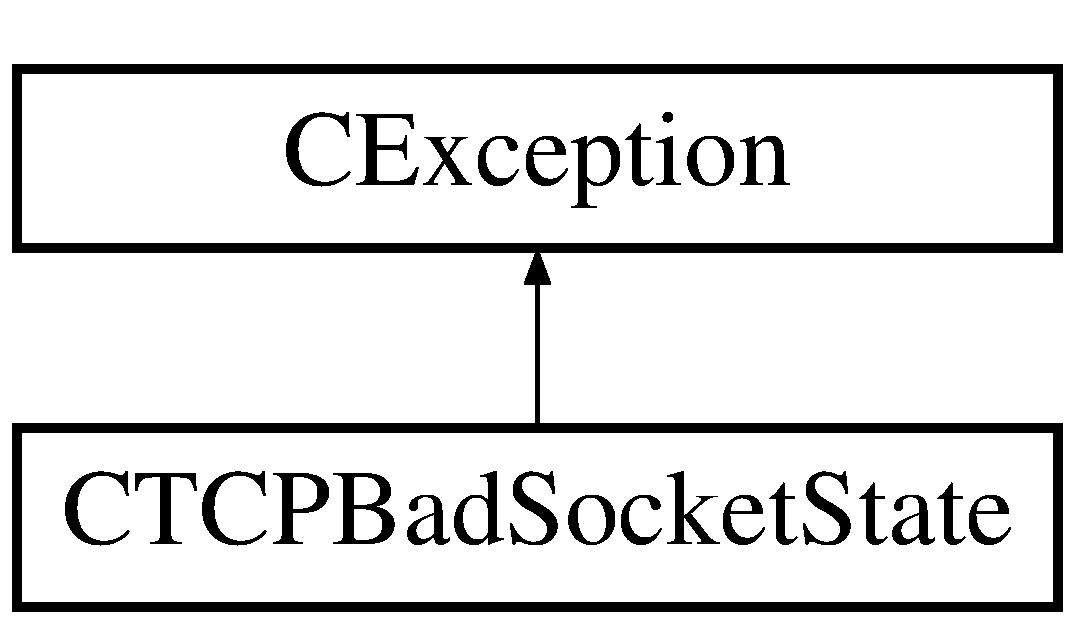
\includegraphics[height=2cm]{classCTCPBadSocketState}
\end{center}
\end{figure}
\subsection*{Public Methods}
\begin{CompactItemize}
\item 
{\bf CTCPBad\-Socket\-State} ({\bf CSocket::State} bad\-State, vector$<$ {\bf CSocket::State} $>$ ok\-States, const char $\ast$p\-Doing)
\item 
{\bf CTCPBad\-Socket\-State} (const CTCPBad\-Socket\-State \&rhs)
\item 
virtual {\bf $\sim$CTCPBad\-Socket\-State} ()
\item 
CTCPBad\-Socket\-State \& {\bf operator=} (const CTCPBad\-Socket\-State \&rhs)
\item 
int {\bf operator==} (const CTCPBad\-Socket\-State \&rhs)
\item 
{\bf CSocket::State} {\bf get\-Bad\-State} () const
\item 
vector$<$ {\bf CSocket::State} $>$ {\bf get\-Valid\-States} () const
\item 
virtual const char $\ast$ {\bf Reason\-Text} () const
\end{CompactItemize}
\subsection*{Protected Methods}
\begin{CompactItemize}
\item 
void {\bf set\-Bad\-State} ({\bf CSocket::State} new\-State)
\item 
void {\bf set\-Valid\-States} (const vector$<$ {\bf CSocket::State} $>$ \&new\-States)
\end{CompactItemize}
\subsection*{Private Attributes}
\begin{CompactItemize}
\item 
{\bf CSocket::State} {\bf m\_\-Bad\-State}
\begin{CompactList}\small\item\em Incorrect state at time of throw.\item\end{CompactList}\item 
vector$<$ {\bf CSocket::State} $>$ {\bf m\_\-Valid\-States}
\begin{CompactList}\small\item\em States which would have been ok.\item\end{CompactList}\item 
string {\bf m\_\-Message}
\begin{CompactList}\small\item\em Full error message built up here.\item\end{CompactList}\end{CompactItemize}


\subsection{Detailed Description}
Encapsulates an exception which will be thrown whenever a {\bf CSocket} {\rm (p.\,\pageref{classCSocket})} member is called when the socket is in an invalid state. The exception recognizes that there may be a list of valid states which the socket can be in and will indicate in the exception message the set of valid states. 



Definition at line 319 of file CTCPBad\-Socket\-State.h.

\subsection{Constructor \& Destructor Documentation}
\index{CTCPBadSocketState@{CTCPBad\-Socket\-State}!CTCPBadSocketState@{CTCPBadSocketState}}
\index{CTCPBadSocketState@{CTCPBadSocketState}!CTCPBadSocketState@{CTCPBad\-Socket\-State}}
\subsubsection{\setlength{\rightskip}{0pt plus 5cm}CTCPBad\-Socket\-State::CTCPBad\-Socket\-State ({\bf CSocket::State} {\em bad\-State}, vector$<$ {\bf CSocket::State} $>$ {\em ok\-States}, const char $\ast$ {\em p\-Doing})}\label{classCTCPBadSocketState_a0}


\char`\"{}Normal Constructor\char`\"{} This constructor is normally used prior to throwing a CTCPBad\-Socket\-State object as an exception.\begin{Desc}
\item[Parameters: ]\par
\begin{description}
\item[{\em 
bad\-State}]- the state of the {\bf CSocket} {\rm (p.\,\pageref{classCSocket})} object which threw the exception which was objectionable. \item[{\em 
ok\-States}]- A vector of states which would have been ok for the socket to have been in at the time it threw. \item[{\em 
p\-Doing}]- A textual description of what the {\bf CSocket} {\rm (p.\,\pageref{classCSocket})} object was asked to do when it detected the invalid state. \end{description}
\end{Desc}


Definition at line 306 of file CTCPBad\-Socket\-State.cpp.

References CSocket::State.\index{CTCPBadSocketState@{CTCPBad\-Socket\-State}!CTCPBadSocketState@{CTCPBadSocketState}}
\index{CTCPBadSocketState@{CTCPBadSocketState}!CTCPBadSocketState@{CTCPBad\-Socket\-State}}
\subsubsection{\setlength{\rightskip}{0pt plus 5cm}CTCPBad\-Socket\-State::CTCPBad\-Socket\-State (const CTCPBad\-Socket\-State \& {\em rhs})}\label{classCTCPBadSocketState_a1}


\char`\"{}Copy constructor\char`\"{} This constructor creates a new object from a 'reference' object. This is used by the compiler to create temporaries, it is also used by throw to copy the exception to a \char`\"{}spot\char`\"{} where it cannot go out of scope as it travels up the call stack in search of a handler.\begin{Desc}
\item[Parameters: ]\par
\begin{description}
\item[{\em 
rhs}]- the reference object copied. \end{description}
\end{Desc}


Definition at line 323 of file CTCPBad\-Socket\-State.cpp.\index{CTCPBadSocketState@{CTCPBad\-Socket\-State}!~CTCPBadSocketState@{$\sim$CTCPBadSocketState}}
\index{~CTCPBadSocketState@{$\sim$CTCPBadSocketState}!CTCPBadSocketState@{CTCPBad\-Socket\-State}}
\subsubsection{\setlength{\rightskip}{0pt plus 5cm}virtual CTCPBad\-Socket\-State::$\sim$CTCPBad\-Socket\-State ()\hspace{0.3cm}{\tt  [inline, virtual]}}\label{classCTCPBadSocketState_a2}




Definition at line 333 of file CTCPBad\-Socket\-State.h.

\subsection{Member Function Documentation}
\index{CTCPBadSocketState@{CTCPBad\-Socket\-State}!getBadState@{getBadState}}
\index{getBadState@{getBadState}!CTCPBadSocketState@{CTCPBad\-Socket\-State}}
\subsubsection{\setlength{\rightskip}{0pt plus 5cm}{\bf CSocket::State} CTCPBad\-Socket\-State::get\-Bad\-State () const\hspace{0.3cm}{\tt  [inline]}}\label{classCTCPBadSocketState_a5}




Definition at line 341 of file CTCPBad\-Socket\-State.h.

References m\_\-Bad\-State, and CSocket::State.\index{CTCPBadSocketState@{CTCPBad\-Socket\-State}!getValidStates@{getValidStates}}
\index{getValidStates@{getValidStates}!CTCPBadSocketState@{CTCPBad\-Socket\-State}}
\subsubsection{\setlength{\rightskip}{0pt plus 5cm}vector$<${\bf CSocket::State}$>$ CTCPBad\-Socket\-State::get\-Valid\-States () const\hspace{0.3cm}{\tt  [inline]}}\label{classCTCPBadSocketState_a6}




Definition at line 343 of file CTCPBad\-Socket\-State.h.

References m\_\-Valid\-States.\index{CTCPBadSocketState@{CTCPBad\-Socket\-State}!operator=@{operator=}}
\index{operator=@{operator=}!CTCPBadSocketState@{CTCPBad\-Socket\-State}}
\subsubsection{\setlength{\rightskip}{0pt plus 5cm}CTCPBad\-Socket\-State \& CTCPBad\-Socket\-State::operator= (const CTCPBad\-Socket\-State \& {\em rhs})}\label{classCTCPBadSocketState_a3}


Assignement... little different from copy construction however:\begin{CompactItemize}
\item 
Any existing members require cleanup if they are dynamic, since we are already fully constructed.\item 
We avoid self assignment.\item 
We return a reference to ourselves after the copy in.\end{CompactItemize}
\begin{Desc}
\item[Parameters: ]\par
\begin{description}
\item[{\em 
rhs}]The right hand side object which is being assigned to us. \end{description}
\end{Desc}


Definition at line 341 of file CTCPBad\-Socket\-State.cpp.

References m\_\-Bad\-State, m\_\-Valid\-States, and CException::operator=().\index{CTCPBadSocketState@{CTCPBad\-Socket\-State}!operator==@{operator==}}
\index{operator==@{operator==}!CTCPBadSocketState@{CTCPBad\-Socket\-State}}
\subsubsection{\setlength{\rightskip}{0pt plus 5cm}int CTCPBad\-Socket\-State::operator== (const CTCPBad\-Socket\-State \& {\em rhs})}\label{classCTCPBadSocketState_a4}


Equality comparison. Returns int indicating if for all practical purposes this is the same as the rhs. m\_\-Message is not compared as it is  inconsequential. \begin{Desc}
\item[Parameters: ]\par
\begin{description}
\item[{\em 
rhs}]The object $\ast$this is being compared to. \end{description}
\end{Desc}


Definition at line 358 of file CTCPBad\-Socket\-State.cpp.

References m\_\-Bad\-State, m\_\-Valid\-States, and CException::operator==().\index{CTCPBadSocketState@{CTCPBad\-Socket\-State}!ReasonText@{ReasonText}}
\index{ReasonText@{ReasonText}!CTCPBadSocketState@{CTCPBad\-Socket\-State}}
\subsubsection{\setlength{\rightskip}{0pt plus 5cm}const char $\ast$ CTCPBad\-Socket\-State::Reason\-Text () const\hspace{0.3cm}{\tt  [virtual]}}\label{classCTCPBadSocketState_a7}


Build up and return a text string describing why the  exception was thrown. This is done from the m\_\-Bad\-State, m\_\-Valid\-States, and base class {\bf Was\-Doing}() {\rm (p.\,\pageref{classCException_a10})} strings. The final string is of the form:

\char`\"{}{\bf CSocket} {\rm (p.\,\pageref{classCSocket})} member called while in state m\_\-Bad\-State, Valid states are m\_\-Valid\-States, {\bf CSocket} {\rm (p.\,\pageref{classCSocket})} was attempting to: {\bf Was\-Doing}() {\rm (p.\,\pageref{classCException_a10})}\char`\"{} 

Reimplemented from {\bf CException} {\rm (p.\,\pageref{classCException_a8})}.

Definition at line 378 of file CTCPBad\-Socket\-State.cpp.

References m\_\-Bad\-State, m\_\-Message, m\_\-Valid\-States, CSocket::State\-Name(), and CException::Was\-Doing().\index{CTCPBadSocketState@{CTCPBad\-Socket\-State}!setBadState@{setBadState}}
\index{setBadState@{setBadState}!CTCPBadSocketState@{CTCPBad\-Socket\-State}}
\subsubsection{\setlength{\rightskip}{0pt plus 5cm}void CTCPBad\-Socket\-State::set\-Bad\-State ({\bf CSocket::State} {\em new\-State})\hspace{0.3cm}{\tt  [inline, protected]}}\label{classCTCPBadSocketState_b0}




Definition at line 349 of file CTCPBad\-Socket\-State.h.

References m\_\-Bad\-State, and CSocket::State.\index{CTCPBadSocketState@{CTCPBad\-Socket\-State}!setValidStates@{setValidStates}}
\index{setValidStates@{setValidStates}!CTCPBadSocketState@{CTCPBad\-Socket\-State}}
\subsubsection{\setlength{\rightskip}{0pt plus 5cm}void CTCPBad\-Socket\-State::set\-Valid\-States (const vector$<$ {\bf CSocket::State} $>$ \& {\em new\-States})\hspace{0.3cm}{\tt  [inline, protected]}}\label{classCTCPBadSocketState_b1}




Definition at line 351 of file CTCPBad\-Socket\-State.h.

References m\_\-Valid\-States.

\subsection{Member Data Documentation}
\index{CTCPBadSocketState@{CTCPBad\-Socket\-State}!m_BadState@{m\_\-BadState}}
\index{m_BadState@{m\_\-BadState}!CTCPBadSocketState@{CTCPBad\-Socket\-State}}
\subsubsection{\setlength{\rightskip}{0pt plus 5cm}{\bf CSocket::State} CTCPBad\-Socket\-State::m\_\-Bad\-State\hspace{0.3cm}{\tt  [private]}}\label{classCTCPBadSocketState_o0}


Incorrect state at time of throw.



Definition at line 323 of file CTCPBad\-Socket\-State.h.

Referenced by get\-Bad\-State(), operator=(), operator==(), Reason\-Text(), and set\-Bad\-State().\index{CTCPBadSocketState@{CTCPBad\-Socket\-State}!m_Message@{m\_\-Message}}
\index{m_Message@{m\_\-Message}!CTCPBadSocketState@{CTCPBad\-Socket\-State}}
\subsubsection{\setlength{\rightskip}{0pt plus 5cm}string CTCPBad\-Socket\-State::m\_\-Message\hspace{0.3cm}{\tt  [private]}}\label{classCTCPBadSocketState_o2}


Full error message built up here.



Definition at line 325 of file CTCPBad\-Socket\-State.h.

Referenced by Reason\-Text().\index{CTCPBadSocketState@{CTCPBad\-Socket\-State}!m_ValidStates@{m\_\-ValidStates}}
\index{m_ValidStates@{m\_\-ValidStates}!CTCPBadSocketState@{CTCPBad\-Socket\-State}}
\subsubsection{\setlength{\rightskip}{0pt plus 5cm}vector$<${\bf CSocket::State}$>$ CTCPBad\-Socket\-State::m\_\-Valid\-States\hspace{0.3cm}{\tt  [private]}}\label{classCTCPBadSocketState_o1}


States which would have been ok.



Definition at line 324 of file CTCPBad\-Socket\-State.h.

Referenced by get\-Valid\-States(), operator=(), operator==(), Reason\-Text(), and set\-Valid\-States().

The documentation for this class was generated from the following files:\begin{CompactItemize}
\item 
{\bf CTCPBad\-Socket\-State.h}\item 
{\bf CTCPBad\-Socket\-State.cpp}\end{CompactItemize}
